\documentclass[11pt]{article}
\usepackage[a4paper,margin=2.6cm]{geometry}
\usepackage[T1]{fontenc}
\usepackage[utf8]{inputenc}
\usepackage{times}
\usepackage{microtype}
\usepackage{booktabs}
\usepackage{graphicx}
\usepackage{amsmath}
\usepackage{xcolor}
\usepackage[numbers,sort&compress]{natbib}
\usepackage[hidelinks]{hyperref}
\usepackage{caption}
\usepackage{enumitem}
\captionsetup{font=small,labelfont=bf}
\setlist{nosep}

\newcommand{\Bfuzzy}{\textsc{Fuzzy}}
\newcommand{\Mcomm}{\textsc{Sonnet-5}}
\newcommand{\Mlocal}{\textsc{Qwen-14B}}

\title{When Does a Language Model Help Code Historical Causes of Death?\\
\large A preregistered comparison of a fuzzy coding dictionary, a local 14B model and a frontier model on ICD10h}

\author{Bart{\l}omiej Nawara\\
Independent researcher, Poland\\
\texttt{[email]}}

\date{September 2026}

\begin{document}
\maketitle

\begin{abstract}
Historical death registers record causes of death in vernacular, misspelled and compound terms (``quinsy'', ``died of grief'', ``congenital chest mischief''). Coding these strings into a modern disease classification is still largely manual work. We ask a narrow question: on chapter-level coding of such strings, does a language model beat a plain fuzzy lookup against a coding dictionary, and if so, where? We use the 3,306 English historic strings of the ICD10h scheme (CC BY 4.0), derive the ICD-10 chapter from each code, hold out 300 strings and use the remaining 3,006 as a dictionary. Before any model was run we fixed the metric, the baselines, a success margin and a kill criterion. A nearest-neighbour lookup by character trigram cosine reaches 0.707 accuracy. Claude Sonnet 5, prompted with only the string and the list of chapters, reaches 0.667 (95\% CI 0.61--0.72); a local Qwen2.5-14B reaches 0.560. The preregistered test therefore fails. The exploratory picture is different. On the 33 held-out strings with no close dictionary neighbour (trigram similarity below 0.5) the dictionary drops to 0.364 while the frontier model holds at 0.758 (paired difference $+0.39$, bootstrap CI 0.21--0.58, exact McNemar $p=0.001$). By macro-F1 the frontier model is also ahead (0.709 vs 0.635). Error analysis shows that a large share of the frontier model's remaining errors are convention errors rather than medical errors: it codes trauma under Injury where ICD10h uses External cause, and it medicalises symptom strings that ICD10h keeps under Ill-defined. Merging Injury into External cause, a post hoc correction, lifts the frontier model to 0.713. A similarity-routed combination (dictionary when a close neighbour exists, model otherwise) reaches 0.750 at the preregistered cut and 0.780 at the best post hoc threshold. We release code, cached outputs and derived data. A preregistered memorisation probe returned empty outputs for all items and is reported as inconclusive.
\end{abstract}

\section{Introduction}

John Graunt met this problem in 1662. Building the first quantitative analysis of the London Bills of Mortality, he found that the causes of death had been written down by untrained parish ``searchers'' in whatever words came to hand, and he had to decide ``whether any credit at all were to be given to their Distinguishments'' \citep{graunt1662}. He settled for lay categories a non-expert could tell apart. The searchers are long gone. The strings they and their successors left behind are still with us, in the millions, and every historical demographer who wants to compare mortality across places and periods has to map them, one by one, onto a coherent classification. Alter and Carmichael observe that there is no key to the translation \citep{alter1999classifying}. The ICD10h scheme \citep{reid2024icd10h} and the SHiP coding effort \citep{janssens2021ship} exist because the work is not done.

The standard tool is a coding dictionary: a list of historic strings paired with codes, which a coder consults, and which software can consult by fuzzy string matching. Dictionaries have a well-known failure mode. They only know the strings they contain. A term that is spelled differently, phrased as an event rather than a disease, or simply absent, gets either no answer or the wrong one from its nearest lexical neighbour. The obvious candidate capability that a large language model might bring is medical and lexical knowledge that generalises to strings the dictionary has never seen.

Whether that capability shows up in practice is an empirical question, and one that is easy to answer badly. Language models are strong on the strings that any method gets right, which inflates aggregate accuracy, and weak on conventions specific to one coding scheme, which deflates it. Aggregate numbers alone will not say whether the model earns its place. This paper is a small, preregistered attempt to answer the question cleanly.

We make the following contributions.
\begin{enumerate}
  \item A chapter-level benchmark on the public ICD10h English historic strings, with a deterministic split, a strong fuzzy dictionary baseline, and a preregistered primary endpoint, success margin and kill criterion (Section~\ref{sec:methods}).
  \item Measured results for a frontier model (Claude Sonnet 5) and a local open-weight model (Qwen2.5-14B) under a minimal prompt with no dictionary access (Section~\ref{sec:results}). On the preregistered endpoint the frontier model loses to the dictionary.
  \item An exploratory analysis that locates where each instrument helps: the dictionary on strings with close neighbours, the frontier model on novel strings and on rare chapters (Sections~\ref{sec:split}--\ref{sec:perchapter}).
  \item An error analysis showing that much of the frontier model's deficit is convention, not medicine, and a similarity-routed hybrid that exceeds both instruments (Sections~\ref{sec:convention}--\ref{sec:routing}).
\end{enumerate}

The primary result is negative and we report it as such. The secondary results are, in our view, the useful ones, and we mark them as exploratory throughout.

\section{Related work}

The closest prior work is \citet{pedersen2024coding}, who evaluate GPT-3.5, GPT-4 and Llama~2 on full ICD-10 code assignment for the HiCaD dataset of 19,361 Scottish and English death register entries from 1861--1901. GPT-4 assigned the correct code for 83\% of causes; a supervised classifier trained on labelled data reached 89\%. They also report that all models did better on terms still in use than on archaic ones. Our study differs in three ways. We code at the chapter level rather than the full code, so the task is coarser but the label set is small enough for a prompt. We use the published ICD10h exemplar strings rather than register entries, so the benchmark is fully reproducible from a CC BY file. And we compare against a dictionary lookup rather than a trained classifier, because a dictionary is what a coding team actually has before any model is involved, and it needs no labelled training run.

For modern clinical text, \citet{soroush2024poor} and \citet{boyle2023automated} report that off-the-shelf language models are weak at exact ICD code assignment and tend to be more useful for coarse categorisation or as retrieval-augmented components. Our chapter-level framing sits at the coarse end of that spectrum.

The ICD10h scheme itself \citep{reid2024icd10h} extends ICD-10 (2016 version) \citep{who2016icd10} with additional codes for archaic terms and ships an exemplar list of historic strings with codes, which is the file we use. The SHiP project \citep{janssens2021ship} pursues a compatible international coding system. Character $n$-gram similarity as a fuzzy matching primitive goes back at least to \citet{kondrak2005ngram}. Our reporting discipline follows the preregistration logic of \citet{nosek2018prereg}: the primary endpoint and its threshold were fixed before any model output was seen.

\section{Data and task}
\label{sec:data}

\paragraph{Source.} We use the ``English language historic strings'' file of ICD10h, version 2024.2 \citep{reid2024icd10h}, licensed CC BY 4.0. It contains 3,306 historic cause-of-death strings, each with an ICD10h code. The strings are short: in the held-out set, 38 are one word, 166 two words, 66 three words, and 30 longer, with a maximum of eight.

\paragraph{Labels.} From each ICD10h code we derive the ICD-10 chapter from the code's letter and two-digit block: A--B Infectious, C and D00--D48 Neoplasm, D50--D89 Blood, E Endocrine/metabolic, F Mental, G Nervous, H00--H59 Eye, H60--H95 Ear, I Circulatory, J Respiratory, K Digestive, L Skin, M Musculoskeletal, N Genitourinary, O Pregnancy, P Perinatal, Q Congenital, R Ill-defined, S--T Injury, V--Y External cause, Z Factors, U Special. Twenty chapters occur in the data; 18 occur in the held-out set. The Injury chapter (S--T) never occurs, in either the dictionary or the test set. The ICD10h strings file carries a separate \texttt{ICD10hInjury} column for the nature-of-injury code, so the primary code for a traumatic death is its external cause. This matters for the error analysis in Section~\ref{sec:convention}. We nonetheless offered all 22 chapter names to the models, because we fixed the label list from the ICD-10 chapter structure before inspecting the data, and removing a chapter after seeing that it was empty would have been exactly the kind of post hoc adjustment we wanted to avoid.

\paragraph{Split.} Strings were de-duplicated case-insensitively, shuffled with seed 0, and the first 300 held out as the test set. The remaining 3,006 form the dictionary. The test set's chapter distribution is skewed: Infectious 46, External cause 37, Ill-defined 31, Neoplasm 28, Digestive 26, Circulatory 24, Genitourinary 24, Respiratory 15, Nervous 14, Skin 13, Musculoskeletal 13, Perinatal 7, Pregnancy 6, Congenital 5, Mental 4, Ear 3, Endocrine/metabolic 3, Blood 1.

\paragraph{Task.} Given a historic string, predict its chapter. The primary metric is accuracy on the 300 held-out strings. We also report macro-F1 over the 18 chapters present in the test set.

\section{Methods}
\label{sec:methods}

\subsection{Baselines}

\textbf{Majority.} Always predict the most frequent chapter in the dictionary (Infectious).

\textbf{Fuzzy dictionary (\Bfuzzy).} For a test string, compute the cosine similarity between its set of character trigrams (letters only, lower-cased) and that of every dictionary string, and return the chapter of the most similar entry. For a query set $Q$ and dictionary set $D$ the score is $|Q\cap D|/\sqrt{|Q|\,|D|}$. No training, no tuning, no tie-breaking beyond first occurrence. We record, for each test string, its best similarity to any dictionary entry; this number defines the HARD subset below.

\subsection{Instruments}

Both models receive the same prompt: a one-sentence system instruction describing the task and the period, the historic string, the list of 22 chapter names, and an instruction to reply with exactly one name (full text in Appendix~\ref{app:prompt}). No dictionary entries, no examples and no reasoning traces are given. This is deliberately the weakest reasonable configuration: we want to measure what the model knows, not what it can copy.

\textbf{\Mlocal.} \texttt{qwen2.5:14b} \citep{qwen2.5} served locally through Ollama at its default quantisation, temperature 0, seed 7, 12 output tokens.

\textbf{\Mcomm.} \texttt{claude-sonnet-5} \citep{anthropic2026sonnet5}, called through the authenticated Claude Code command-line interface in print mode with tools disabled. The interface exposes no temperature control, so each string was queried once and the raw output cached. All 300 outputs were exact chapter names; no parsing fallback was needed. The run took 22 minutes on 9 August 2026.

Free-text outputs are mapped to chapters by exact match, then case-insensitive substring match in a fixed order, then a short alias list; an unparseable output would be scored as Ill-defined. This fallback fired zero times for either model.

\subsection{Preregistered protocol}

The following was written down before any model call.
\begin{itemize}
  \item Primary endpoint: accuracy on the 300 held-out strings, with a 95\% bootstrap confidence interval (1,000 resamples, seed 0) \citep{efron1993bootstrap}.
  \item Kill criterion: \Mcomm{} must exceed the best baseline by at least $+0.05$ accuracy. With \Bfuzzy{} at 0.707 the target was 0.757. Failure yields the verdict \textsc{killed}.
  \item Secondary, explicitly not part of the kill test: accuracy on the HARD subset, defined as test strings whose best dictionary similarity is below 0.5, and the comparison between the commercial and the local model.
  \item No threshold moves after seeing model numbers.
\end{itemize}
The 0.5 cut was chosen as a round number before the similarity distribution was inspected. It produced $n=33$ HARD strings (median best similarity in the test set is 0.71; the 10th percentile is 0.49).

\subsection{Memorisation probe}
\label{sec:probe-method}

ICD10h is public and a frontier model may have seen it. Chapter-level correctness on ``cholera'' is medical knowledge and is not a threat. Recall of the scheme's idiosyncratic extended codes (``A00.900'' for ``asiatic cholera'') would be. We preregistered a probe: ask \Mcomm{} for the exact ICD10h code of the first 30 test strings, giving one worked example in the prompt, and score exact-code and first-three-character matches. A non-trivial exact-match rate (above 0.15) would flag likely exposure.

\subsection{Supplementary analyses}

Everything in this subsection was added after the primary result and is exploratory. We compute: paired bootstrap confidence intervals (5,000 resamples) and exact McNemar tests \citep{mcnemar1947} for the difference between \Bfuzzy{} and \Mcomm{} on the full, HARD and non-HARD sets; accuracy within bins of best dictionary similarity; per-chapter F1; confusion counts; accuracy after merging the Injury chapter into External cause; and a routed hybrid that returns the dictionary's answer when the best similarity is at least $\tau$ and the model's answer otherwise, for $\tau$ from 0 to 1. The hybrid at $\tau=0.5$ uses only the preregistered cut and needs no tuning; the best $\tau$ is chosen on the test set and is an upper bound, not an estimate.

\section{Results}
\label{sec:results}

\subsection{Primary endpoint}

Table~\ref{tab:main} gives the headline numbers. \Bfuzzy{} reaches 0.707 (CI 0.653--0.757). \Mcomm{} reaches 0.667 (CI 0.610--0.720), a difference of $-0.040$ against a required $+0.05$. The preregistered verdict is \textsc{killed}. \Mlocal{} reaches 0.560 and is below the dictionary on every cut except the HARD tail.

\begin{table}[t]
\centering
\caption{Chapter-level results on the 300 held-out ICD10h strings. HARD: best char-trigram similarity to any dictionary string below 0.5. Bootstrap 95\% CIs in brackets. Bold marks the best in each column.}
\label{tab:main}
\footnotesize
\setlength{\tabcolsep}{4pt}
\begin{tabular}{lcccc}
\toprule
Method & Acc.\ all ($n{=}300$) & Acc.\ HARD ($n{=}33$) & Acc.\ non-HARD ($n{=}267$) & Macro-F1 \\
\midrule
Majority & 0.153 [0.113, 0.193] & 0.091 [0.000, 0.212] & 0.161 [0.120, 0.206] & 0.015 \\
\Bfuzzy{} & \textbf{0.707} [0.653, 0.757] & 0.364 [0.212, 0.545] & \textbf{0.749} [0.697, 0.801] & 0.635 [0.558, 0.703] \\
\Mlocal{} & 0.560 [0.507, 0.617] & 0.576 [0.424, 0.727] & 0.558 [0.502, 0.618] & 0.568 [0.499, 0.635] \\
\Mcomm{} & 0.667 [0.613, 0.720] & \textbf{0.758} [0.606, 0.879] & 0.655 [0.603, 0.712] & \textbf{0.709} [0.630, 0.768] \\
\bottomrule
\end{tabular}
\end{table}

The full-set difference between \Mcomm{} and \Bfuzzy{} is not distinguishable from zero: paired bootstrap CI $[-0.11, +0.03]$, exact McNemar $p=0.30$ (63 strings the dictionary gets right and the model wrong, 51 the other way). So the honest statement is that on this benchmark as constructed, a fuzzy lookup and a frontier model with no dictionary access are roughly tied on aggregate accuracy, with the dictionary numerically ahead, and the model does not clear the margin we demanded.

\subsection{The split by dictionary similarity}
\label{sec:split}

The aggregate hides two opposite regimes (Figure~\ref{fig:bins}). On the 267 non-HARD strings, which have a dictionary neighbour at similarity 0.5 or above, \Bfuzzy{} beats \Mcomm{} by $0.094$ (CI $[-0.169, -0.022]$ for model minus dictionary, McNemar $p=0.015$; 62 vs 37 discordant). On the 33 HARD strings the direction reverses and the effect is large: \Mcomm{} is ahead by $0.394$ (CI $[0.212, 0.576]$, McNemar $p=0.001$; 14 vs 1 discordant). The dictionary collapses to 0.364 there because its nearest neighbour is lexically misleading: ``quinsy'' matches ``insanity'', ``synovitis'' matches ``otitis'', ``beaten with iron bar'' matches ``lithiasis''. The model has no such problem; it knows what quinsy is.

\begin{figure}[t]
\centering
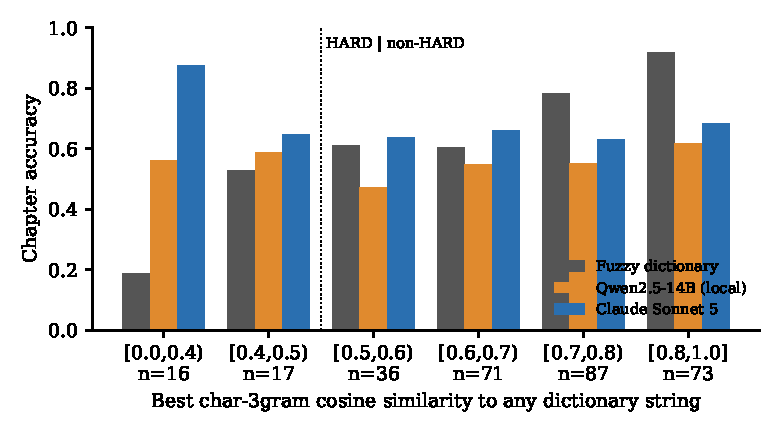
\includegraphics[width=0.8\linewidth]{figs/acc_by_similarity.pdf}
\caption{Accuracy as a function of the test string's best character-trigram similarity to the dictionary. The dictionary's accuracy rises monotonically with similarity, from 0.19 in the lowest bin to 0.92 in the 0.8--1.0 bin. Both models are flat. The frontier model is at 0.875 in the lowest bin ($n=16$).}
\label{fig:bins}
\end{figure}

Figure~\ref{fig:bins} shows the finer structure. Dictionary accuracy is almost a linear function of similarity, from 0.19 in the $[0,0.4)$ bin to 0.92 in the $[0.8,1.0]$ bin. Both models are flat across bins, at roughly 0.55--0.60 for \Mlocal{} and 0.63--0.68 for \Mcomm{}, with one exception: in the lowest bin, the 16 strings least like anything in the dictionary, \Mcomm{} reaches 0.875. The crossover between dictionary and frontier model is somewhere in the 0.6--0.7 similarity range. HARD is small ($n=33$) and its CI is wide, but the finding is not a fluke of the cut: it reappears in every bin below 0.6 and in the discordant-pair counts.

\subsection{Per-chapter behaviour}
\label{sec:perchapter}

Macro-F1 favours \Mcomm{} (0.709 vs 0.635), though the paired difference, $0.074$ with CI $[-0.017, 0.156]$, does not exclude zero. Figure~\ref{fig:chapters} gives the per-chapter picture. The dictionary is strongest on the large chapters with many near-duplicate strings: Infectious (0.80 vs 0.61), External cause (0.84 vs 0.69), Digestive (0.77 vs 0.61), Circulatory (0.83 vs 0.72), Nervous (0.76 vs 0.61) and Ill-defined (0.55 vs 0.26). The frontier model wins on Neoplasm (0.96 vs 0.89), Genitourinary (0.82 vs 0.54), Respiratory (0.77 vs 0.49), Perinatal, Congenital, Mental, Ear and Endocrine. These are the chapters where either the vocabulary is technical enough that medical knowledge dominates (neoplasms, respiratory terms) or the chapter is rare enough that the dictionary has few neighbours to offer. The local model is roughly competitive with the frontier model on Neoplasm, Musculoskeletal, Genitourinary and Skin, and far behind on External cause (0.05), for a reason we give next.

\begin{figure}[t]
\centering
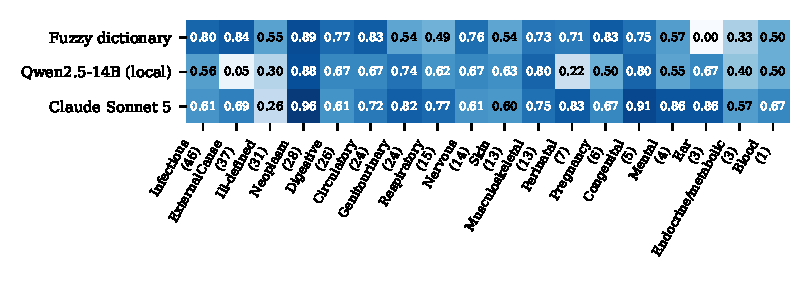
\includegraphics[width=\linewidth]{figs/per_chapter_f1.pdf}
\caption{Per-chapter F1 on the held-out set (chapter support in parentheses). Chapters ordered by test frequency.}
\label{fig:chapters}
\end{figure}

\subsection{Where the frontier model loses: convention, not medicine}
\label{sec:convention}

The confusion counts (Table~\ref{tab:confusions}) are dominated by three cells, and none of them is a medical mistake.

\begin{table}[t]
\centering
\caption{Most frequent confusions (gold $\to$ predicted) for each instrument on the held-out set.}
\label{tab:confusions}
\small
\begin{tabular}{llr@{\hskip 2em}llr}
\toprule
\multicolumn{3}{c}{\Bfuzzy{}} & \multicolumn{3}{c}{\Mcomm{}} \\
\cmidrule(r){1-3}\cmidrule(l){4-6}
Gold & Predicted & $n$ & Gold & Predicted & $n$ \\
\midrule
Genitourinary & Ill-defined & 8 & External cause & Injury & 14 \\
Infectious & Respiratory & 4 & Infectious & Digestive & 11 \\
Infectious & Digestive & 3 & Ill-defined & Digestive & 9 \\
Infectious & Ill-defined & 3 & Ill-defined & Circulatory & 5 \\
Ill-defined & Respiratory & 3 & Skin & Infectious & 5 \\
Skin & Ill-defined & 3 & Infectious & Nervous & 4 \\
Neoplasm & Respiratory & 3 & Circulatory & Nervous & 3 \\
\bottomrule
\end{tabular}
\end{table}

\paragraph{External cause versus Injury.} \Mcomm{} labels 14 gold External-cause strings as Injury: ``fracture skull supposed'', ``amputation arm'', ``compound fracture'', ``blow to the head'', ``carbolic acid'', ``suicide poisoning vitriol''. In ICD-10 these strings describe the nature of an injury (S--T) and its external cause (V--Y) at once; the ICD10h file records the external cause in the primary column and the nature of injury in a separate \texttt{ICD10hInjury} column. A model that has not read the ICD10h manual cannot know which of the two ICD10h treats as primary. \Mlocal{} makes the same choice 31 times, which is where its External-cause F1 of 0.05 comes from. The dictionary never predicts Injury because no dictionary entry carries it. If Injury is merged into External cause, a correction we did not preregister and report only as a diagnostic, \Mcomm{} rises from 0.667 to 0.713 and \Mlocal{} from 0.560 to 0.657, and the frontier model edges past the dictionary on the full set. Nothing about this correction involves medicine. It is a one-line convention of the target scheme.

\paragraph{Ill-defined.} ICD10h keeps symptom-only strings under R (Ill-defined): ``loss of blood'', ``shortness of breath'', ``gripes'', ``jaundice'', ``icterus'', ``dropsy abdomen''. The frontier model prefers an organ system, calling these Digestive (9), Circulatory (5), Infectious (3) and so on. It predicted Ill-defined for only 8 of 300 strings against 31 gold and 45 dictionary predictions. The dictionary over-predicts Ill-defined and still does better on that chapter, because the historic coders' reluctance to commit is encoded in the neighbouring entries, and the dictionary copies it.

\paragraph{Infectious versus Digestive.} Eleven gold-Infectious strings are called Digestive: ``gastro enteritis acute'', ``entero-colitis'', ``bowels catarrh acute'', ``tuberculosis bowels acute'', ``catarrhal jaundice''. ICD-10 places infectious gastroenteritis under A09 and intestinal tuberculosis under A18, in Chapter I, and ICD10h follows. A clinician reading ``gastro enteritis'' thinks of the gut. The chapter structure thinks of the pathogen. Again the model is not wrong about the disease; it is wrong about the filing cabinet.

Together these three cells account for 34 of the frontier model's 100 errors. The dictionary's errors, by contrast, are lexical accidents spread thinly across many cells, the largest being Genitourinary strings matched to Ill-defined neighbours.

\subsection{A similarity-routed hybrid}
\label{sec:routing}

The two instruments fail in different places, which suggests routing on the one quantity we have for free: the best dictionary similarity. Return the dictionary's chapter if that similarity is at least $\tau$, otherwise the model's. Figure~\ref{fig:hybrid} traces accuracy over $\tau$. At the preregistered cut $\tau=0.5$, which involves no tuning on the test set, the hybrid with \Mcomm{} reaches 0.750 (macro-F1 0.689), above both components and just short of the 0.757 target. The best post hoc threshold, $\tau=0.65$, gives 0.780, and the curve is above 0.75 for every $\tau$ between 0.5 and 0.8. With \Mlocal{} as the fallback the hybrid peaks at 0.730 at $\tau=0.5$. An oracle that takes either component's answer whenever one is right reaches 0.877, so roughly half the remaining headroom between the routed hybrid and the oracle is in strings where the two disagree and the similarity does not tell which to trust.

\begin{figure}[t]
\centering
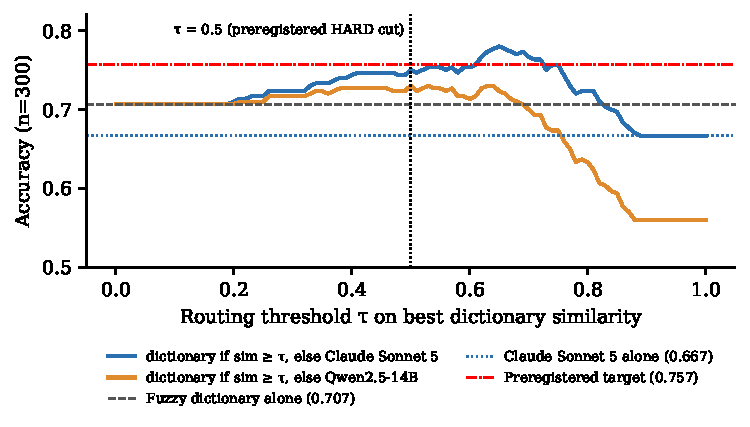
\includegraphics[width=0.8\linewidth]{figs/hybrid_routing.pdf}
\caption{Accuracy of a routed hybrid that answers from the dictionary when the best similarity is at least $\tau$ and from the model otherwise. The value at $\tau=0.5$ is tuning-free; the peak at $\tau=0.65$ is selected on the test set and is an upper bound.}
\label{fig:hybrid}
\end{figure}

We stress the status of these numbers. The $\tau=0.5$ hybrid is a legitimate, tuning-free system and its 0.750 is a fair estimate. The 0.780 is what one gets by picking the best of 101 thresholds on 300 items and should not be quoted as an expected accuracy.

\subsection{Memorisation probe: inconclusive}
\label{sec:probe}

The probe returned an empty string for all 30 items. The exact-match rate is therefore 0.000, but so is the base rate of any answer at all, and we cannot tell a model that does not know the codes from a model that declined to guess them, or from an interface artefact in how the command-line tool handled the prompt. We had preregistered a reading of ``low exact-match means the chapter accuracy rests on general knowledge''; that reading assumed the model would produce codes. It did not. We report the probe because it was preregistered and we treat the memorisation question as open. Two considerations reduce the concern without settling it. First, nothing in the chapter-level results looks like recall: the model's errors are systematic convention errors of exactly the kind a model that had memorised ICD10h's codes would not make, since the codes encode the convention. Second, the strings on which the model does best are the ones least like anything in the published file.

\section{Discussion}

\paragraph{The dictionary is the right baseline, and it is hard to beat.} A character-trigram lookup with no training reaches 0.707 on this task. Anyone proposing a model for historical cause-of-death coding should have to beat that, on the same split, before claiming anything. Most of the held-out strings are near-duplicates of strings the scheme's authors already coded, and on those a model that has not seen the scheme is guessing a convention that the dictionary simply copies.

\paragraph{The model helps exactly where the dictionary cannot.} On the tail of novel strings the frontier model is far ahead, and the effect is large enough to survive a small $n$. This is the case that motivated the study: the string nobody has coded before. The demographer's practical question is not ``model or dictionary'' but ``what do I do with the 10\% of strings the dictionary returns garbage for'', and the answer, on this evidence, is to ask the model.

\paragraph{Most of the model's deficit is not a knowledge gap.} Three convention errors account for a third of the frontier model's mistakes, and one of them, Injury versus External cause, can be removed by one sentence in the prompt or one line of post-processing. We did not do that here, because the point was to measure the untouched instrument. A model given the ICD10h manual, or a handful of coded examples per chapter, would plausibly close most of this gap. That is a different experiment, and a cheap one.

\paragraph{Scale matters on this task.} The local 14B model is below the dictionary everywhere except the novel tail, and below the frontier model on every cut. Medical vocabulary in obsolete registers is not something a mid-sized open model has much of. This is one of the tasks where the frontier model's advantage is about what it knows rather than how it reasons.

\paragraph{Why preregister a benchmark this small.} Because the temptation to move the goalposts was real. The HARD result is the interesting one, it was the secondary endpoint, and it would have been easy to lead with it. Fixing the primary endpoint in advance meant the headline had to be the negative result, and the exploratory findings had to be labelled as such. We think this makes the paper more useful, not less.

\section{Limitations}

The label space is the ICD-10 chapter, 20 classes, not the full ICD10h code. The benchmark tests broad categorisation. The data are the ICD10h exemplar strings, curated by the scheme's authors, and not raw register entries; real registers are noisier, longer and more repetitive, and the dictionary would likely do better on them, not worse, since repetition favours lookup. The HARD subset has 33 strings and its confidence intervals are wide; the effect size is large but a replication on a bigger tail set is needed before the $+0.39$ is quoted as a stable number. The frontier model was sampled once per string with no temperature control, through a command-line interface rather than an API; run-to-run variation is unmeasured. The memorisation probe failed to produce data. Only one dataset, one language and one period are covered. The hybrid's best threshold is selected on the test set. We evaluated one prompt, chosen to be minimal; better prompts exist and we did not look for them.

\section{Conclusion}

On chapter-level coding of the ICD10h English historic strings, a fuzzy dictionary lookup (0.707) is not beaten by a frontier language model prompted with the string alone (0.667), and the preregistered test fails. On the 33 strings with no close dictionary neighbour the same model reaches 0.758 against the dictionary's 0.364. A third of the model's errors are coding conventions of the target scheme rather than medical errors. A similarity-routed combination of the two reaches 0.750 with no tuning. The evidence supports a division of labour: dictionary first, model for the tail, and a short lesson in the scheme's conventions for the model before it starts.

\section*{Reproducibility and data statement}

Code, the derived split, cached raw model outputs and the analysis script that produces every number and figure in this paper are at \url{https://github.com/th00masml/cause-of-death-coding} \citep{nawara2026repo}. The ICD10h strings file is not redistributed; it is CC BY 4.0 and downloadable from the Cambridge repository \citep{reid2024icd10h}, and \texttt{prepare.py} rebuilds the split deterministically from it. Derived files are shared under CC BY 4.0 with attribution to Reid, Garrett and Hiltunen Maltesdotter. The Graunt quotation is from the public-domain Hull edition. Recomputing all results from the cached outputs takes seconds and needs only NumPy and Matplotlib.

\section*{Acknowledgements}

The author thanks the ICD10h authors for releasing the historic strings under an open licence, which made a fully reproducible benchmark possible.

\bibliographystyle{plainnat}
\bibliography{refs}

\appendix

\section{Prompt}
\label{app:prompt}

System instruction (both models):
\begin{quote}\small\ttfamily\raggedright\sloppy
You are a medical coder assigning historical (17th-20th century) causes of death to broad modern disease categories. Reply with exactly one category name from the given list and nothing else.
\end{quote}
User message, with \texttt{\{s\}} the historic string:
\begin{quote}\small\ttfamily\raggedright\sloppy
Historic cause of death: "\{s\}"\\[2pt]
Assign it to ONE of these categories:\\
Infectious, Neoplasm, Blood, Endocrine/metabolic, Mental, Nervous, Eye, Ear, Circulatory, Respiratory, Digestive, Skin, Musculoskeletal, Genitourinary, Pregnancy, Perinatal, Congenital, Ill-defined, Injury, ExternalCause, Factors, Special\\[2pt]
Answer with exactly one category name.
\end{quote}
For \Mlocal{} the system instruction and user message were concatenated into a single prompt. The memorisation probe prompt was: \emph{In the ICD10h historic cause-of-death coding scheme, every historic term has a specific code (for example ``asiatic cholera'' is coded A00.900). Give the exact ICD10h code for this term. Reply with only the code. Term: ``\{s\}''}.

\section{Output parsing}

Model output is lower-cased and stripped, then matched to a chapter by exact name, then by substring in the fixed chapter order above, then by a small alias table (``cancer'' $\to$ Neoplasm, ``heart'' $\to$ Circulatory, ``external'' $\to$ ExternalCause, and similar). The substring pass is order-dependent: \Mlocal{} once answered ``Injury, ExternalCause'' and once ``Toxicological/ExternalCause'', both scored as Injury because Injury precedes ExternalCause in the list. \Mcomm{} produced a bare chapter name on all 300 items.

\section{The HARD subset}
\label{app:hard}

The 33 held-out strings with best dictionary similarity below 0.5, with the gold chapter, the dictionary's prediction and the frontier model's prediction, are listed in Table~\ref{tab:hard}.

\begin{table}[h]
\centering
\caption{All 33 HARD strings. Bold marks a correct prediction.}
\label{tab:hard}
\scriptsize
\begin{tabular}{llll}
\toprule
String & Gold & \Bfuzzy{} & \Mcomm{} \\
\midrule
quinsy & Respiratory & Mental & \textbf{Respiratory} \\
strophulus & Ill-defined & \textbf{Ill-defined} & Skin \\
glands in the lungs & Respiratory & Ill-defined & \textbf{Respiratory} \\
influence of alcohol & Mental & Respiratory & ExternalCause \\
loss of blood & Ill-defined & Blood & Blood \\
nettle rash & Skin & Ill-defined & \textbf{Skin} \\
knife wound & ExternalCause & \textbf{ExternalCause} & \textbf{ExternalCause} \\
synovitis & Musculoskeletal & Ear & \textbf{Musculoskeletal} \\
want & ExternalCause & Perinatal & Ill-defined \\
teething diarrheoa & Digestive & \textbf{Digestive} & \textbf{Digestive} \\
congenital chest mischief & Congenital & Infectious & \textbf{Congenital} \\
ulceration skin between the shoulders & Skin & \textbf{Skin} & \textbf{Skin} \\
died soon after birth & Perinatal & \textbf{Perinatal} & \textbf{Perinatal} \\
beaten with iron bar & ExternalCause & Genitourinary & \textbf{ExternalCause} \\
ichorrhaemia & Infectious & Ill-defined & Circulatory \\
house fire & ExternalCause & Ill-defined & \textbf{ExternalCause} \\
tumour pelvis & Neoplasm & \textbf{Neoplasm} & \textbf{Neoplasm} \\
not clear & Ill-defined & Skin & \textbf{Ill-defined} \\
died suddenly & Ill-defined & \textbf{Ill-defined} & \textbf{Ill-defined} \\
prurigo & Skin & Infectious & \textbf{Skin} \\
entozoa & Infectious & Respiratory & \textbf{Infectious} \\
noma pudendi & Genitourinary & Skin & Infectious \\
pressure brain & Nervous & \textbf{Nervous} & \textbf{Nervous} \\
gripes & Ill-defined & Respiratory & Digestive \\
myocardial fibrosis & Circulatory & \textbf{Circulatory} & \textbf{Circulatory} \\
died of grief & Mental & ExternalCause & \textbf{Mental} \\
self-inflicted & ExternalCause & Respiratory & \textbf{ExternalCause} \\
dog bite & ExternalCause & \textbf{ExternalCause} & \textbf{ExternalCause} \\
heart irregularity & Circulatory & \textbf{Circulatory} & \textbf{Circulatory} \\
cancrum oris & Infectious & Neoplasm & \textbf{Infectious} \\
shortness of breath & Ill-defined & Perinatal & Respiratory \\
fall of building & ExternalCause & \textbf{ExternalCause} & \textbf{ExternalCause} \\
asystole & Circulatory & Ill-defined & \textbf{Circulatory} \\
\bottomrule
\end{tabular}
\end{table}

\end{document}
